\section{Kryptographische Grundlagen}%
\label{sec:kryptographische_grundlagen}

Kerckhoffsche Annahme: Sicherheit hängt nur von den Schlüsseln ab und nicht vom Unwissen
des kryptographischen Verfahrens.

Grundlegendes Verfahren:
Der Klartext $p$ wird mittels Schlüssel $k$ durch die Verschlüsselungsfunktion $E$ zum
Geheimtext verschlüsselt:
\begin{align*}
  c = E_k(p)
\end{align*}
Dieser Geheimtext wird versendet und vom Empfänger mit der Entschlüsselungsfunktion $D$
und dem Schlüssel $k'$ entschlüsselt, sodass gilt:
\begin{align*}
  D_{k'}(c) = D_{k'}(E_k(p)) = p
\end{align*}
Der Angreifer möchte den Klartext herausfinden und braucht dazu den Schlüssel zum
Entschlüsseln (dies kann der gleiche Schlüssel sein wie zum Verschlüsseln).

Es gibt bspw. folgende Angriffsmodelle:
\begin{itemize}
  \item ciphertext-only
  \item known-plaintext
  \item (adaptive) chosen-plaintext
  \item (adaptive) chosen-ciphertext
\end{itemize}

\subsection{Symmetrische Verschlüsselung}%
\label{sub:symmetrische_verschlusselung}

Hierbei ist der Schlüssel zum Verschlüsseln der gleiche, wie zum Entschlüsseln.
Es gibt je nach Anwendungsfall zwei verschiedene Verfahren:
\begin{itemize}
  \item stream cipher: Stromverschlüsselung.
    Der fortlaufende Klartext wird mittels XOR mit einem Schlüsselstrom
    (normalerweise ein Pseudozufallszahlengenerator) verknüpft.
    Der Seed des Pseudozufallszahlengenerators ist der Schlüssel $k$.
  \item block cipher: Blockverschlüsselung.
    Verschlüsselt den Klartext blockweise mit dem Schlüssel.
    Dabei muss ein Block immer voll gefüllt sein, sodass manchmal Padding nötig ist.
\end{itemize}

Besonderes Verfahren: one-time pad.
Der Schlüsselstrom ist eine reine zufällige Bitfolge, die Absender und Empfänger vorher
kennen.
Der Schlüssel muss genauso lang wie der Klartext sein.
Der Schlüssel darf sich selbst nicht wiederholen.
Dies ist dann bedingungslos sicher.

Praktische Verfahren nutzen wesentlich kürzere Schlüssel.
Diese sind nicht mehr bedingungslos sicher, aber rechnerisch undurchführbar zu brechen.

Beispiel: DES (ist aber unsicher, weil die Schlüssellänge zu kurz ist).

\subsection{Asymmetrische Verschlüsselung}%
\label{sub:asymmetrische_verschlusselung}

Hierbei ist der Schlüssel zum Entschlüsseln $k$ verschieden zum Verschlüsselungsschlüssel
$k'$.
Es ist rechnerisch undurchführbar $k'$ aus $k$ zu ermitteln.
Daher kann $k$ öffentlich gemacht werden (public key).

\subsection{Hybride Verschlüsselung}%
\label{sub:hybride_verschlusselung}

Symmetrische Verschlüsselung ist schnell und asymmetrische Verschlüsselung ist langsam.
Bei symmetrischer Verschlüsselung muss jedoch der Schlüssel übertragen werden.
Lösung: nutze erst asymm. Verschlüsselung um eine Nachricht und Sessionkey zu übertragen
und danach symm. Verschlüsselung für die weitere Kommunikation.
Siehe~\ref{fig:Hybride_Verschlüsselung}.

\begin{figure}[h]
  \centering
  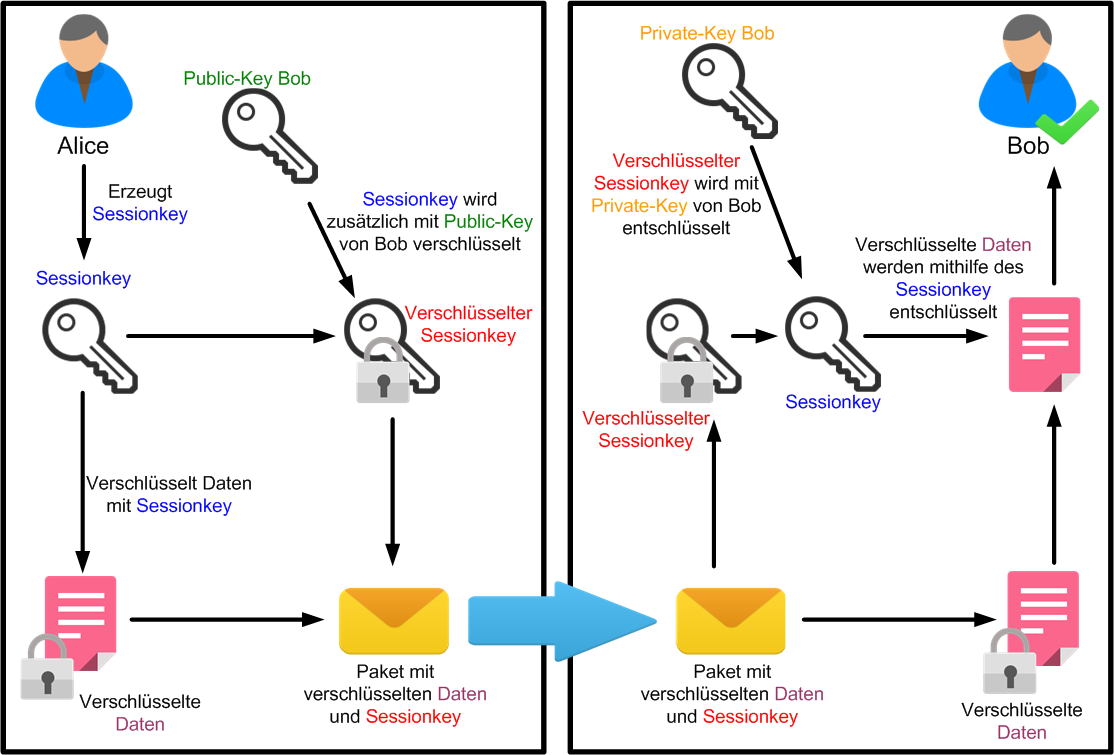
\includegraphics[width=0.9\linewidth]{bilder/Hybride_Verschluesselung.png}
  \caption{Hybride Verschlüsselung}
  \label{fig:Hybride_Verschlüsselung}
\end{figure}

\subsection{Kryptographische Hashfunktionen}%
\label{sub:kryptographische_hashfunktionen}

Eine Hashfunktion $h$ macht aus einer Nachricht beliebiger Länge einen Hashwert mit fester
Länge.

Anforderungen:
\begin{itemize}
  \item Einweg: sei $y$ ein gegebener Hashwert, dann ist es rechnerisch undurchführbar
    eine Nachricht $x$ zu finden, sodass $h(x) = y$ gilt.
  \item schwacher Kollisionswiderstand: sei $x$ eine Nachricht, dann ist es rechnerisch
    undurchführbar eine andere Nachricht $x'$ zu finden, sodass $h(x) = h(x')$ gilt.
  \item (starker) Kollisionswiderstand: es ist rechnerisch undurchführbar zwei Nachrichten
    $x$ und $x'$ zu finden, sodass $h(x) = h(x')$ gilt.
\end{itemize}

Aufgrund des Geburtstagsparadoxons werden viele Bits gebraucht, damit Kollisionen
vermieden werden.
Sei $n$ die Anzahl der möglichen Hashwerte.
Dann kann eine Kollision bei $\sqrt{n}$ Nachrichten mit einer Wahrscheinlichkeit größer
als $0.5$ gefunden werden.
Bei einer Größe der Ausgabe von $h$ von $64$ Bits ist $\sqrt{n} = 232$ zu klein.
Die Größe der Ausgabe sollte mindestens $128$ oder besser $160$ sein.

Ein Problem bei Krypto im Netzwerk ist: die Nachrichten bzw. Pakete haben alle die gleiche
Struktur (z.\,B. Header, IP-Adressen, etc.) und enthalten damit teilweise bekannte
Klartexte.
Dadurch kann ein Angreifer möglicherweise Rückschlüsse auf den Schlüssel ziehen oder
verschlüsselte Blöcke durch eigene ersetzen.
Um das zu verhindern werden die verschlüsselten Blöcke miteinander durch \emph{cipher
block chaining} verbunden.

Hashfunktionen werden auch zum Signieren von Nachrichten verwendet (Nachricht hashen,
Hashwert verschlüsseln und anhängen).

Zum Schlüsselaustausch wird Diffie-Hellman verwendet:
\begin{enumerate}
  \item Alice und Bob einigen sich auf eine (große) Primzahl $p$ und $g < p$, wobei $g$
    ein Erzeuger von $\Integers_p$ ist.
    Auch Eve darf $p$ und $g$ kennen.
  \item Alice und Bob wählen zufällig eine Zahl $a$ bzw. $b$. aus $\{1, \ldots, p-1\}$
    aus, welche geheim bleiben.
  \item Alice berechnet ihren öffentlichen Schlüssel $A = g^a \mod p$ und sendet $A$ an
    Bob.
    Bob berechnet analog $B = g^b \mod p$ und sendet $B$ an Alice.
  \item Alice berechnet den gemeinsamen Schlüssel $K_1 = B^a \mod p$
    und Bob analog $K_2 = A^b \mod p$.

    Es gilt:
    \begin{align*}
      K_1 & = B^a \mod p = (g^b \mod p)^a \mod p = (g^b)^a \mod p = g^{ba} \mod p\\
      K_2 & = A^b \mod p = (g^a \mod p)^b \mod p = (g^a)^b \mod p = g^{ab} \mod p\\
      K_1 & = g^{ba} \mod p = g^{ab} \mod p = K_2
    \end{align*}
\end{enumerate}
Bei DH ist ein man in the middle Angriff möglich.

\subsection{Zertifikate}%
\label{sub:zertifikate}

Ein Zertifikat ist eine Datenstruktur bestehend aus:
\begin{itemize}
  \item dem öffentlichen Schlüssel
  \item Name des Besitzers des öffentlichen Schlüssels
  \item Name des Herausgebers
  \item Datum der Herausgabe
  \item Ablaufdatum
  \item mögliche andere Daten
  \item Signatur des Herausgebers
\end{itemize}

Zertifikate werden von einer Certification Authority (CA) herausgegeben, welcher vertraut
werden muss.
Zertifikate werden durch Certificate Directories verteilt, denen nicht vertraut werden
muss.
Eine Certificate Chain enthält Ketten von CAs und eigentlich muss man nur der Root-CA
vertrauen.
